
\begin{figure}[H]
	\centering
	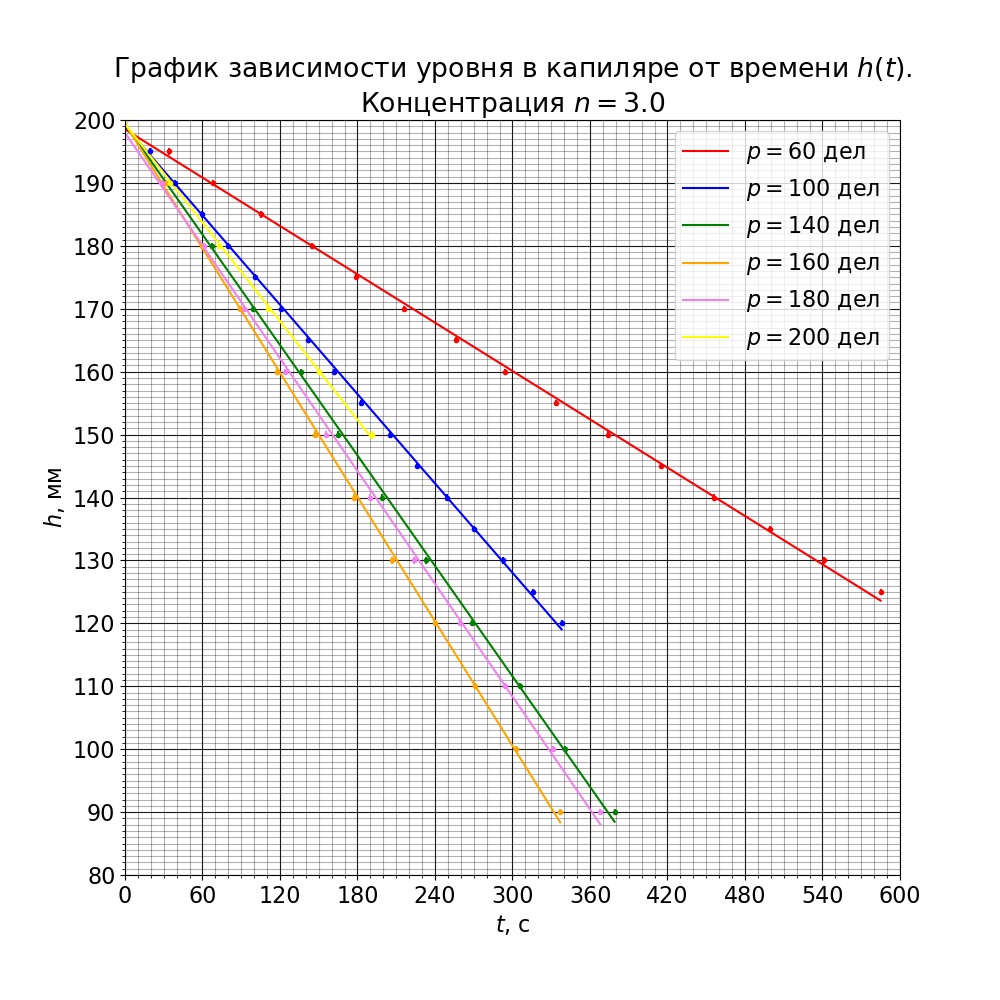
\includegraphics[width=1 \textwidth]{../plots/graph_h_t_0.png}
\end{figure}

Методом наименьших квадратов проведём наилучшую прямую $h~=~at~+~b$.

\begin{tabular}[t]{|c|c|c|c|c|}
\hline
$p$, дел & $a$, $\frac{мм}{с}$ & $\sigma_a$, $\frac{мм}{с}$ & $b$, мм & $\sigma_b$, мм \\ 
\hline
60 & -0,128 & 0,001 & 198,5 & 0,4 \\ 
100 & -0,237 & 0,001 & 199,0 & 0,3 \\ 
140 & -0,293 & 0,002 & 199,3 & 0,5 \\ 
160 & -0,329 & 0,003 & 199,4 & 0,5 \\ 
180 & -0,299 & 0,003 & 198,0 & 0,7 \\ 
200 & -0,261 & 0,003 & 199,4 & 0,4 \\ 
\hline
\end{tabular}

\begin{figure}[H]
	\centering
	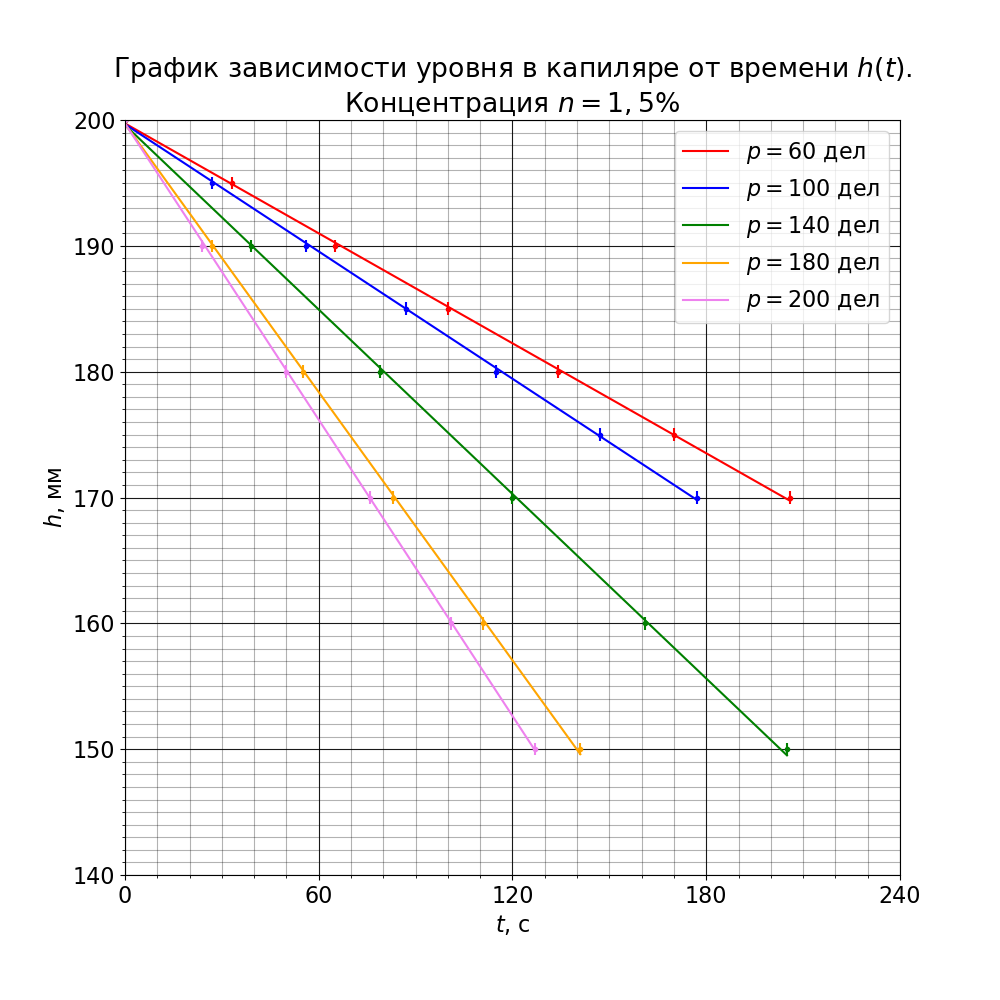
\includegraphics[width=1 \textwidth]{../plots/graph_h_t_1.png}
\end{figure}

Методом наименьших квадратов проведём наилучшую прямую $h~=~at~+~b$.

\begin{tabular}[t]{|c|c|c|c|c|}
\hline
$p$, дел & $a$, $\frac{мм}{с}$ & $\sigma_a$, $\frac{мм}{с}$ & $b$, мм & $\sigma_b$, мм \\ 
\hline
60 & -0,146 & 0,001 & 199,7 & 0,2 \\ 
100 & -0,169 & 0,002 & 199,7 & 0,2 \\ 
140 & -0,244 & 0,002 & 199,6 & 0,3 \\ 
180 & -0,355 & 0,003 & 199,7 & 0,2 \\ 
200 & -0,392 & 0,002 & 199,7 & 0,2 \\ 
\hline
\end{tabular}

\begin{figure}[H]
	\centering
	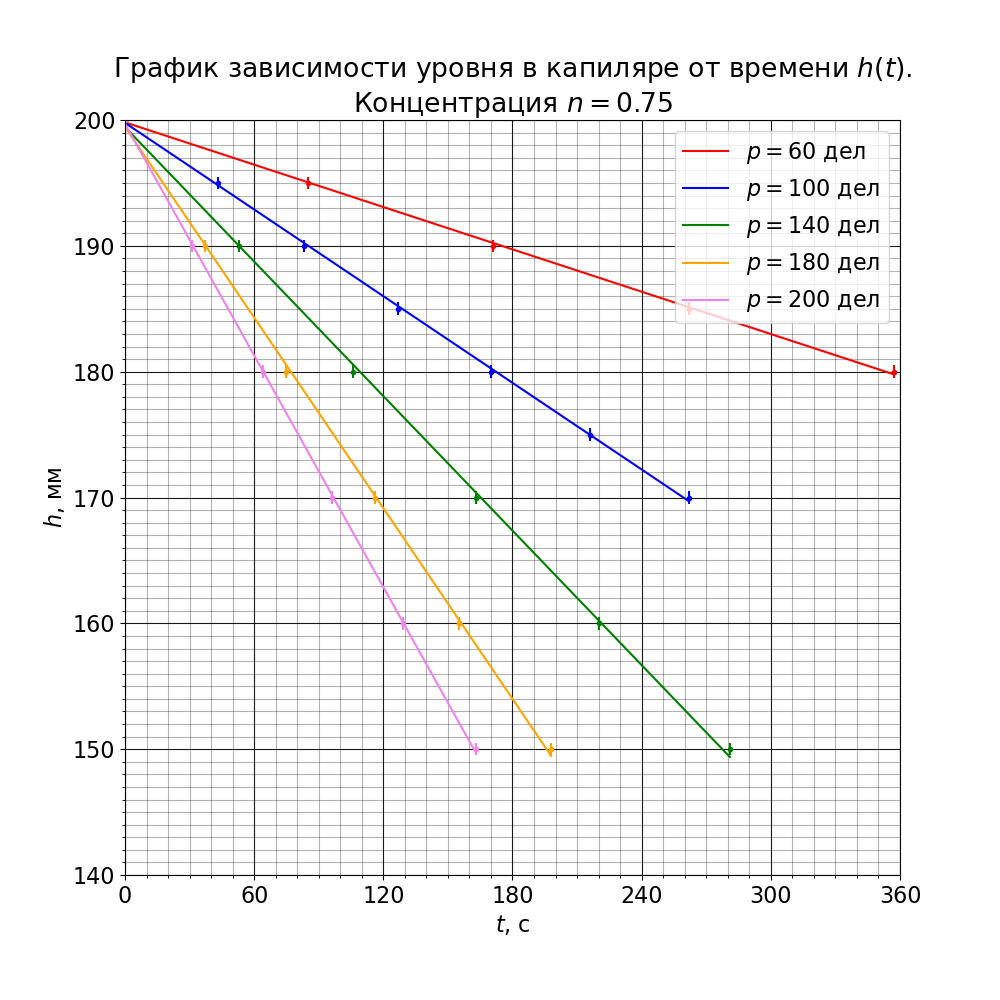
\includegraphics[width=1 \textwidth]{../plots/graph_h_t_2.png}
\end{figure}

Методом наименьших квадратов проведём наилучшую прямую $h~=~at~+~b$.

\begin{tabular}[t]{|c|c|c|c|c|}
\hline
$p$, дел & $a$, $\frac{мм}{с}$ & $\sigma_a$, $\frac{мм}{с}$ & $b$, мм & $\sigma_b$, мм \\ 
\hline
60 & -0,056 & 0,001 & 199,8 & 0,2 \\ 
100 & -0,115 & 0,001 & 199,8 & 0,2 \\ 
140 & -0,178 & 0,002 & 199,4 & 0,4 \\ 
180 & -0,253 & 0,003 & 199,5 & 0,4 \\ 
200 & -0,307 & 0,002 & 199,7 & 0,2 \\ 
\hline
\end{tabular}

\begin{figure}[H]
	\centering
	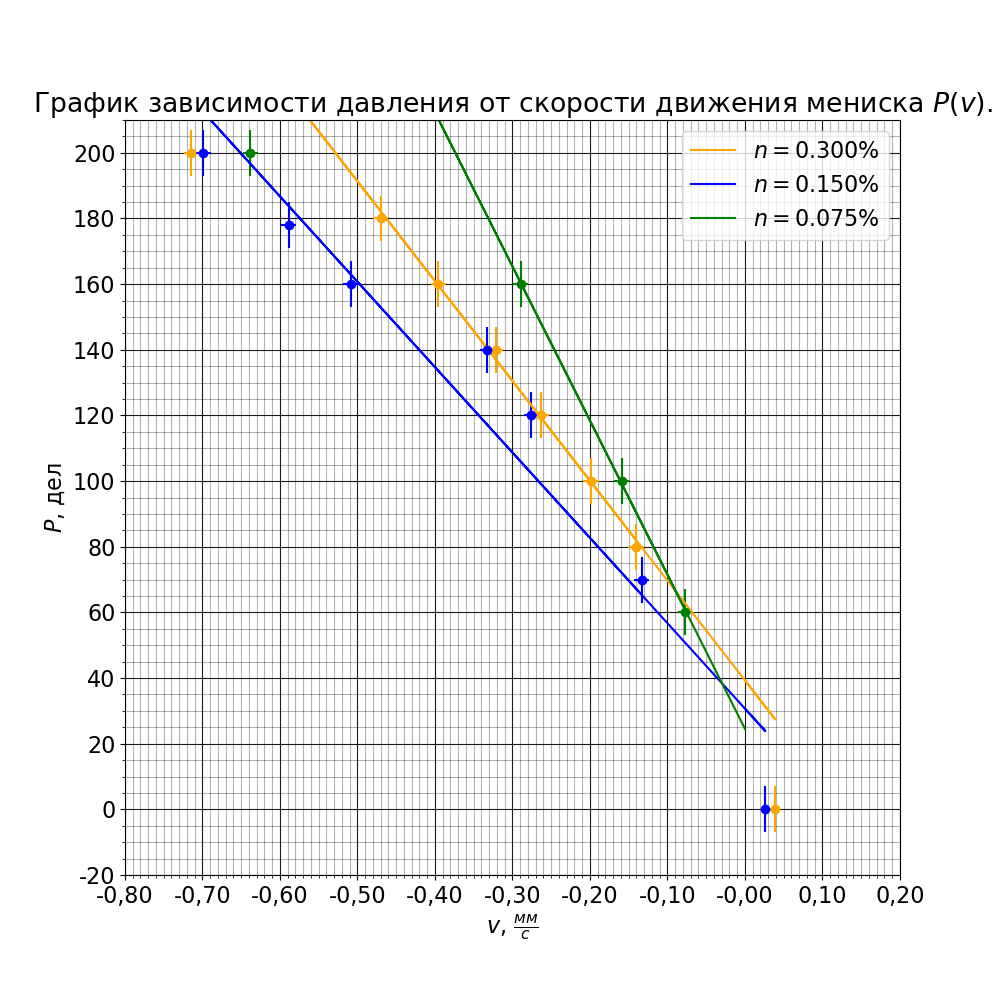
\includegraphics[width=1 \textwidth]{../plots/graph_v_p.png}
\end{figure}

Методом наименьших квадратов проведём наилучшую прямую $v~=~ap~+~b$.

\begin{tabular}[t]{|c|c|c|c|c|}
\hline
$n$, \% & $a$, $\frac{мм}{с \cdot дел}$ & $\sigma_a$, $\frac{мм}{с \cdot дел}$ & $b$, $\frac{мм}{с}$ & $\sigma_b$, $\frac{мм}{с}$ \\ 
\hline
<<<<<<< Updated upstream
3,00 & -0,0021 & 0,0004 & -0,0135 & 0,0400 \\ 
1,50 & -0,0019 & 0,0002 & -0,0064 & 0,0344 \\ 
0,75 & -0,0018 & 0,0001 & 0,0574 & 0,0144 \\ 
=======
0,30 & -0,0033 & 0,0001 & 0,1280 & 0,0114 \\ 
0,15 & -0,0036 & 0,0004 & 0,0908 & 0,0556 \\ 
0,08 & -0,0021 & 0,0000 & 0,0521 & 0,0041 \\ 
>>>>>>> Stashed changes
\hline
\end{tabular}

\begin{figure}[H]
	\centering
	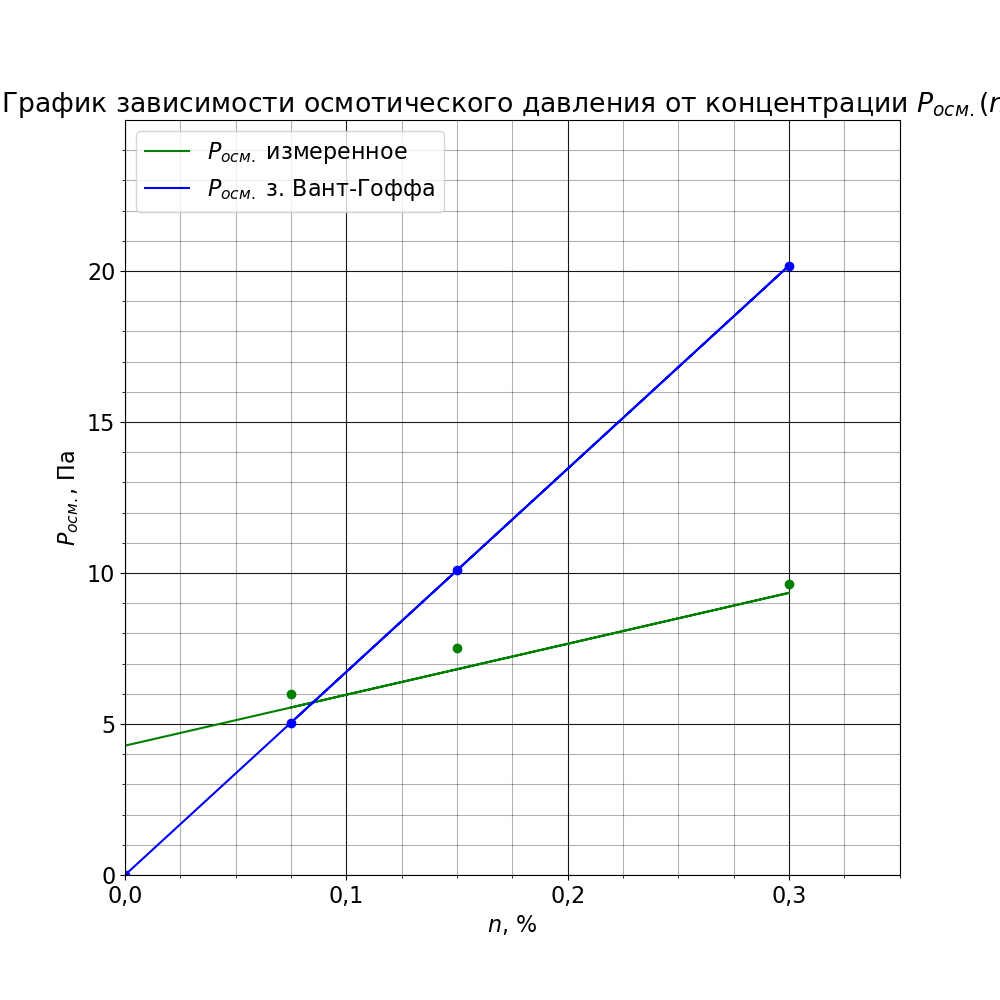
\includegraphics[width=1 \textwidth]{../plots/graph_p_osm_n.png}
\end{figure}

Методом наименьших квадратов по измеренных точкам проведём наилучшую прямую $P~=~an~+~b$. Также построим график зависимости осмотического давления от концентрации по закону Вант-Гоффа.

\begin{tabular}[t]{|c|c|c|c|}
\hline
$a$, $\frac{Па}{\%}$ & $\sigma_a$, $\frac{Па}{\%}$ & $b$, Па & $\sigma_b$, Па \\ 
\hline
16870,9881 & 5182,5088 & 4282,0069 & 1028,3722 \\ 
\hline
\end{tabular}